\chapter{Holistic Evaluation}

We deployed Smart Zone in an 8-room, single story, 1200 square foot residential
building shown in Figure~\ref{fig:floorplan}. The HVAC system setup is overlaid
in order to show the position of vents, ducts, and the central air handler.

\begin{figure}[ht]
  \centering
  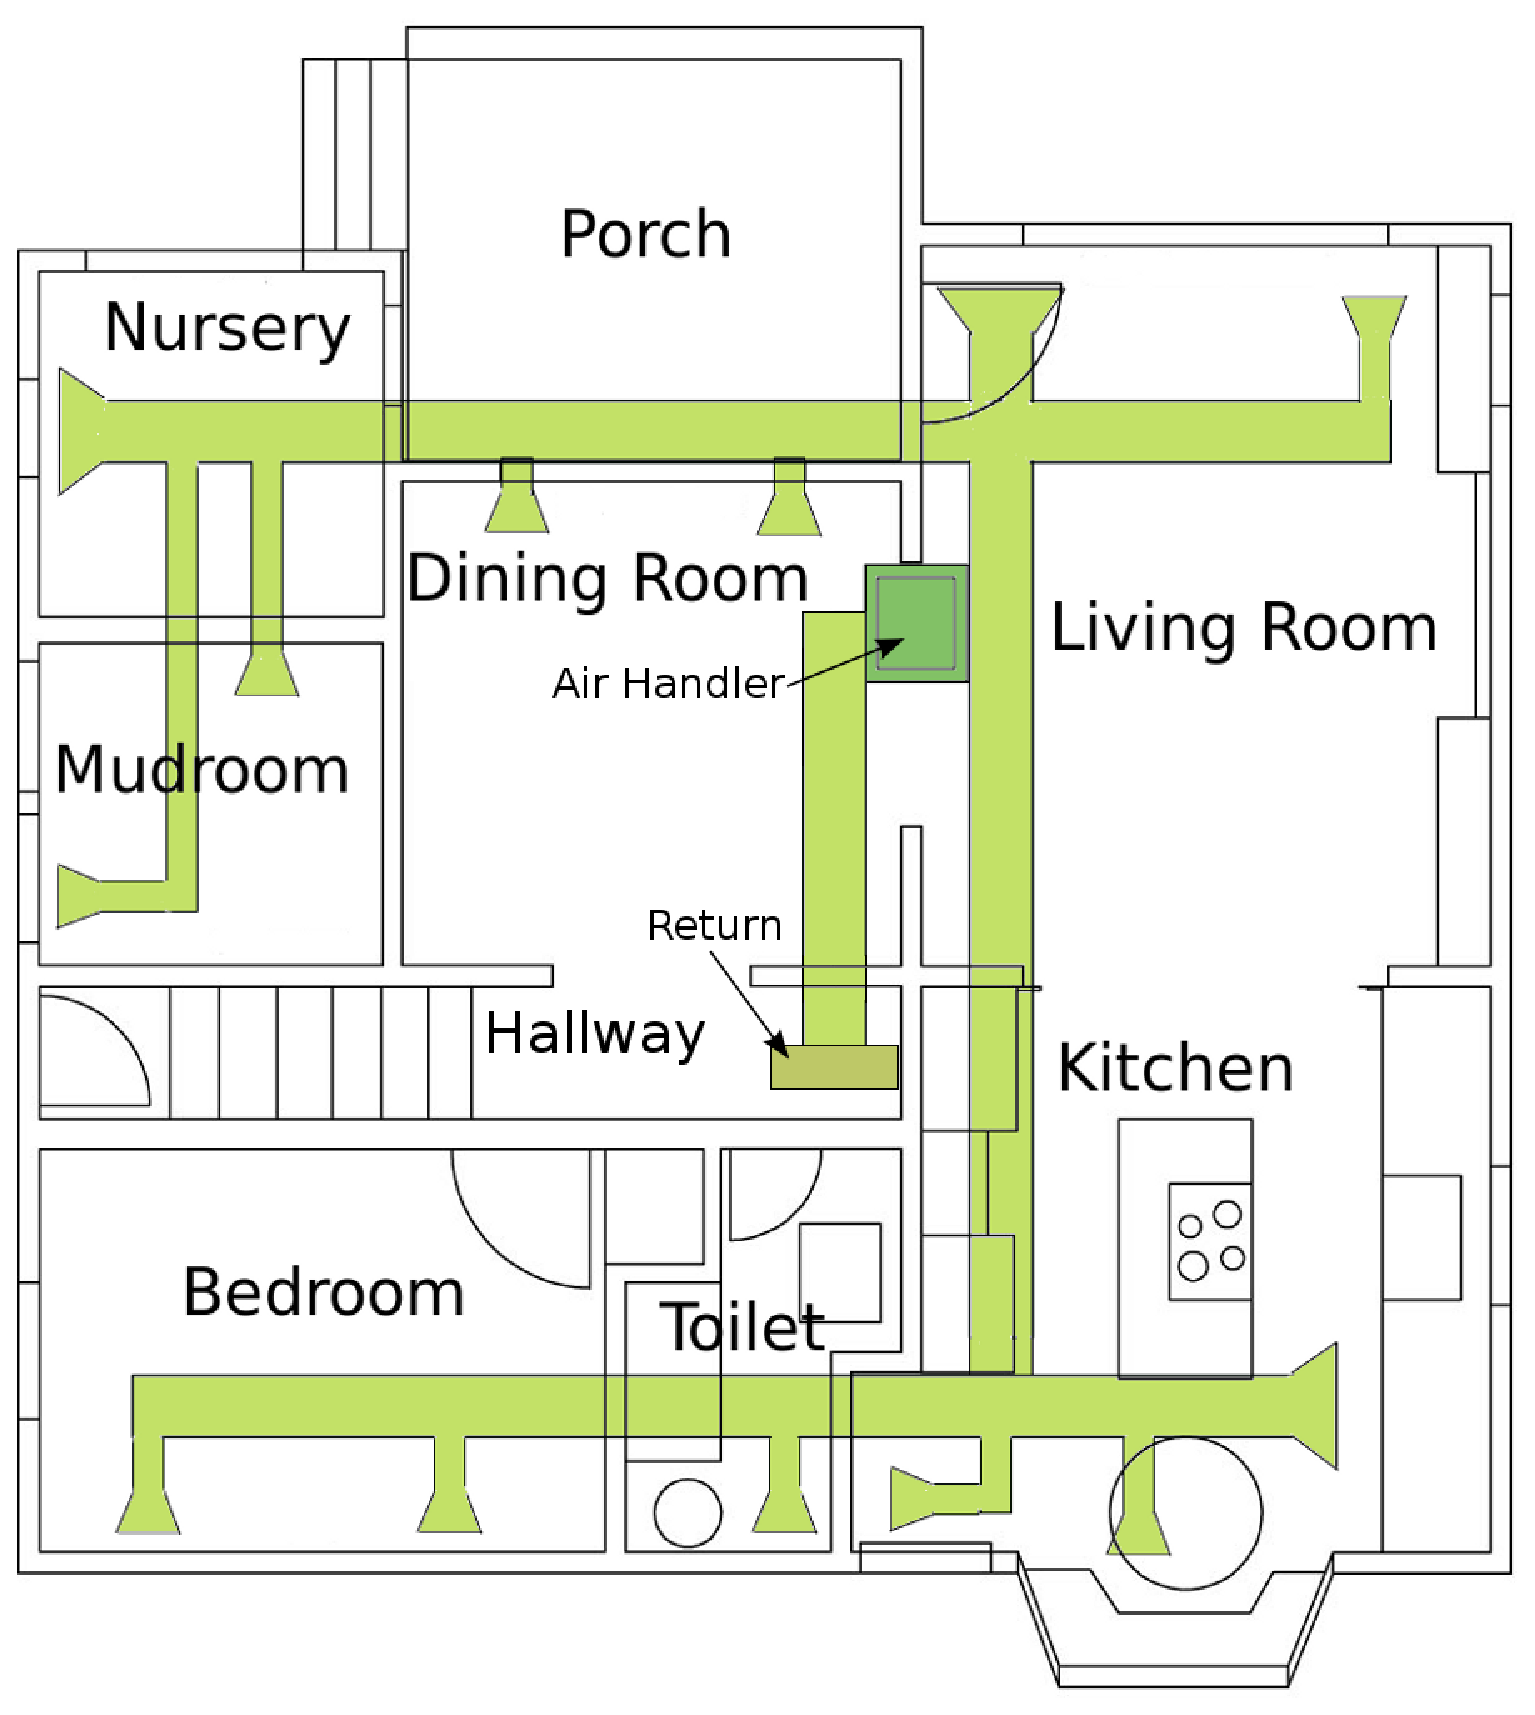
\includegraphics[width=0.6\columnwidth]{fig/floorplan-mechanical.eps}
  \caption[The Residence in which Smart Zone is Evaluated]{The residence in
    which Smart Zoning is implemented with green ducts terminating in
    registers that can be opened or closed.}
  \label{fig:floorplan}
\end{figure}

\section{Static Zoning}
Our initial evaluations involved statically zoning the house into two zones as
shown in Figure~\ref{fig:floorplan}. The red zone composed of the living room,
dining room, and kitchen is actively conditioned between 8:00 AM and 9:30 PM
while the blue zone composed of the bedroom, nursery, toilet, and mudroom is
conditioned between midnight and 8:00 AM. Between 9:30 PM and midnight the whole
house is conditioned.  We compare this approach to conditioning of the whole
house using an off-the shelf programmable thermostat manufactured by {\em
  BAYweb}~\cite{bayweb}.  In both cases, the setpoint temperature of the house
is controlled by the occupants. This means that the experiments measure the
energy required to keep the occupants comfortable with both systems, as opposed
to keeping the space at a particular setpoint.

\begin{figure}[ht]
  \centering
  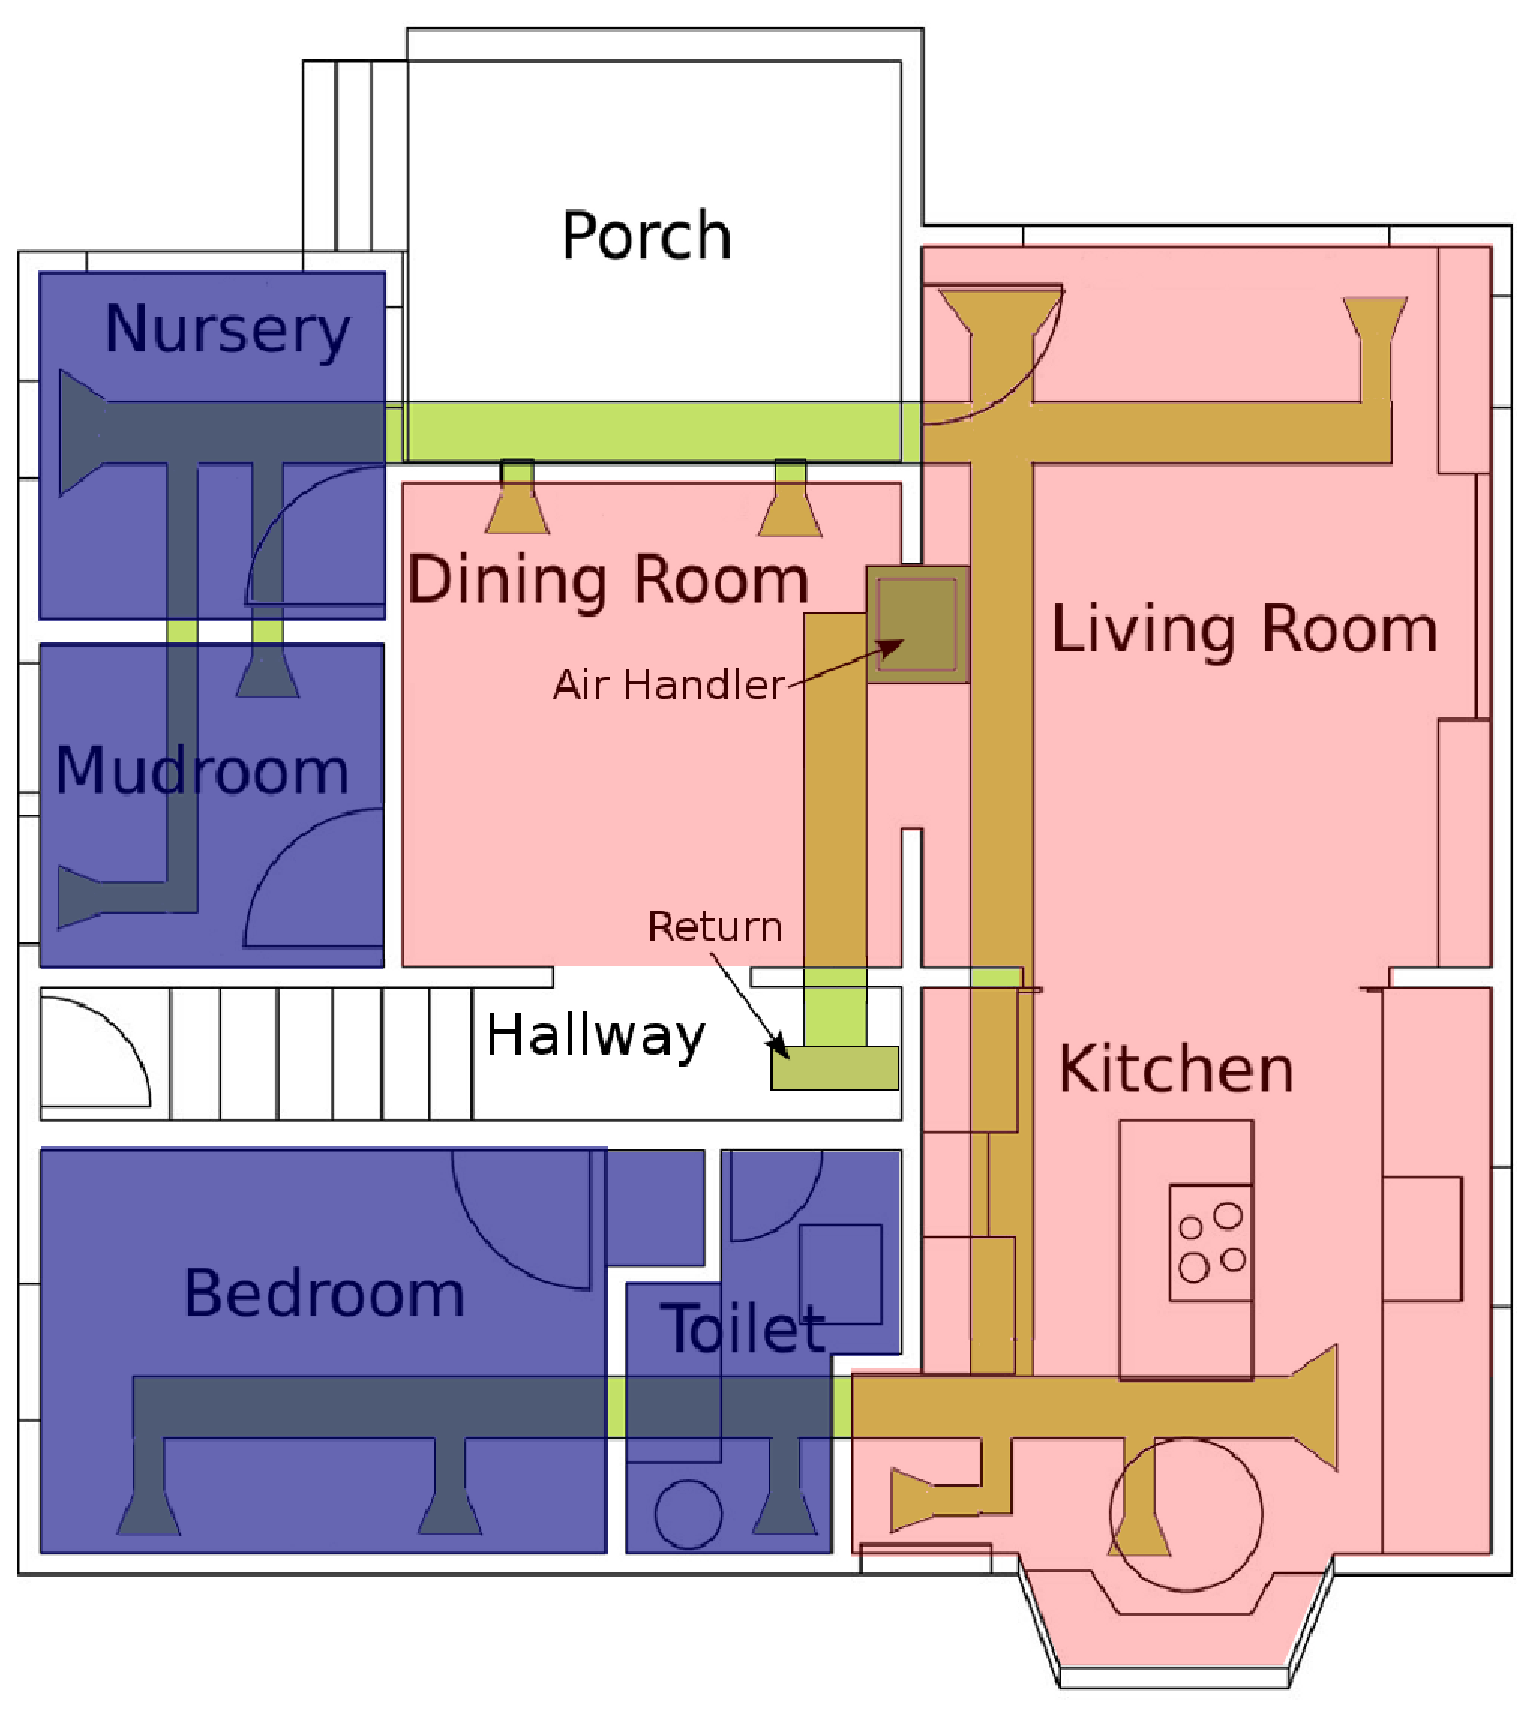
\includegraphics[width=0.6\columnwidth]{fig/floorplan-mechanicalZoned.eps}
  \caption[Static Zones]{The rooms that
    compose Zone 1 are shaded in light red and the rooms that compose Zone 2 are
    shaded in dark blue.}
  \label{fig:floorplan}
\end{figure}

In order to minimize the effect of changing whether patterns on energy
consumption, we alternated control of the HVAC system between the single-zoned
whole house control and the sub-zoned controller over a twenty day period, such
that each system ran every second daty.  Both systems executed for a total of 10
days. The energy consumed by all systems in the house was monitored using The
Energy Detective (TED)~\cite{Energy} real-time in-home energy management system
and the amount of energy used by the HVAC system was deduced using the operation
logs generated by the BAYweb thermostat.

Figure~\ref{fig:energy} shows the energy consumed in conditioning a house using
sub-zoning and whole house conditioning. This graph indicates that whole-house
conditioning consumed 20.5\% more energy than our prototype implementation of
room-level zoning, on average.  The actual energy consumption for each day is
also shown as a scatter plot, with the average temperature of for that day on
the x-axis, the energy consumed on the y-axis, and the control algorithm shown
as the color of the scatter point.

\label{subsec:experimentalResults}
\begin{figure}[ht]
  \centering
  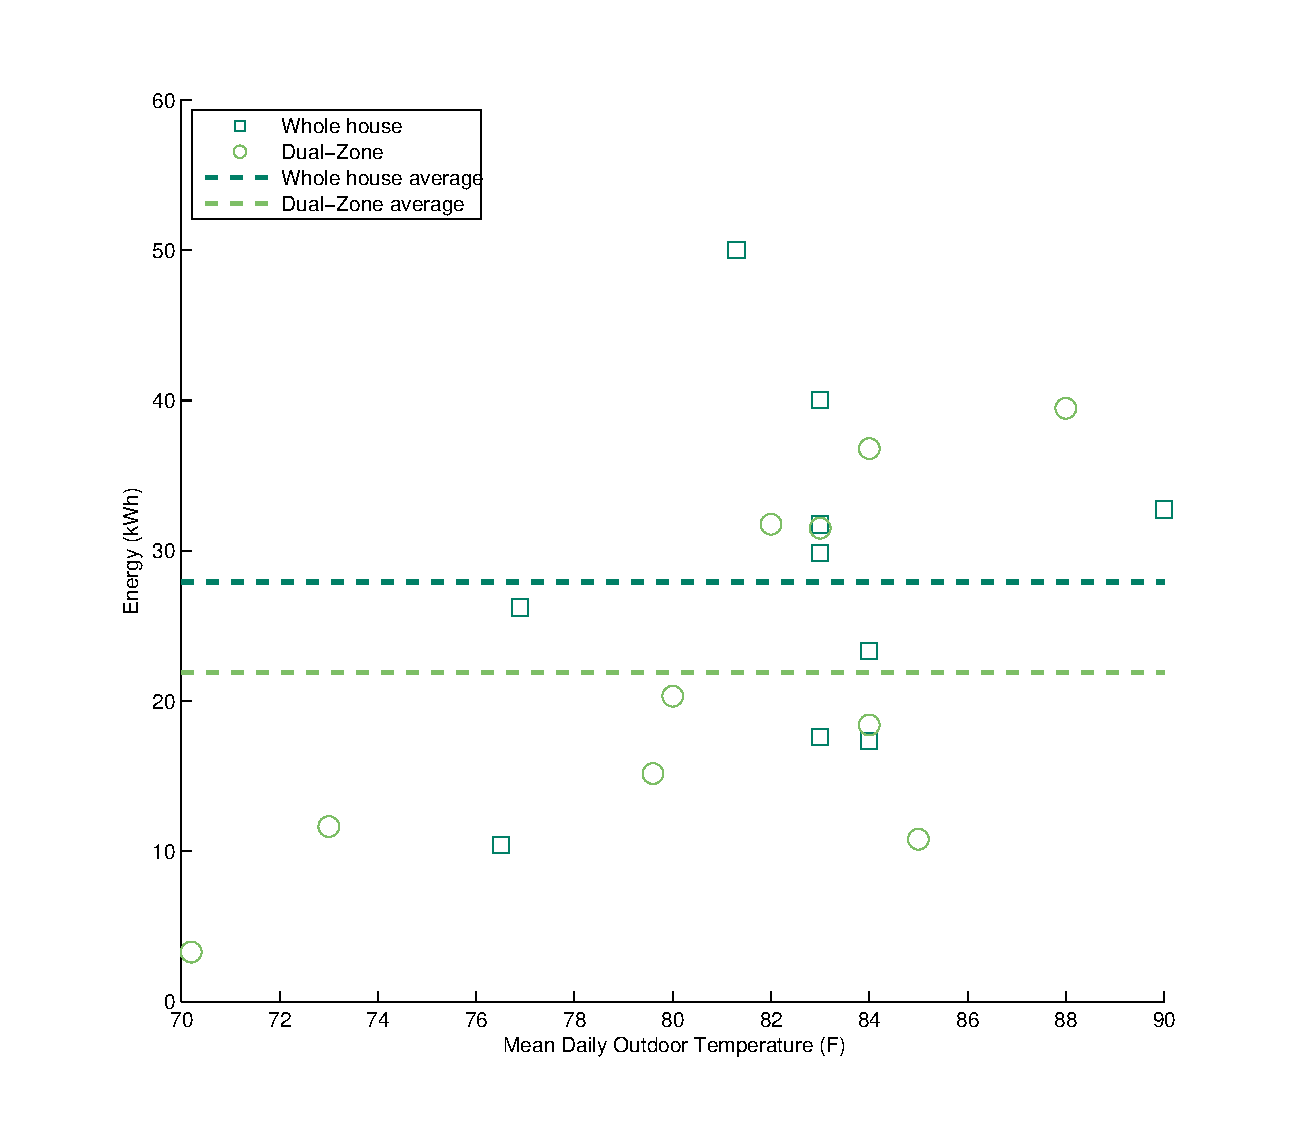
\includegraphics[width=1.0\columnwidth]{fig/meanEnergyScatter.eps}
  \caption[Energy Usage of Static Zones vs. Whole House Conditioning]{Our implementation of room-level zoning uses 20.5\% less energy than
    whole house cooling on average. The dotted lines indicate the average energy
    used over the experimental period.}
  \label{fig:energy}
\end{figure}

Figure~\ref{fig:houseTempRes} shows how the temperature of several rooms in
different zones vary as the temperature in the active zone was dropped from 76
to 72 degrees.  In this graph, the bottom three lines shown the temperature of
conditioned rooms over time while the top two lines show the temperature of
unconditioned rooms.  Although some leakage is evident, particularly into the
top line, the temperatures of the unconditioned rooms remains substantially
higher than the conditioned rooms.  These temperature traces explains how
room-level zoning is able to save energy by reducing the size of the space that
must be conditioned.

\begin{figure}[ht]
  \centering
  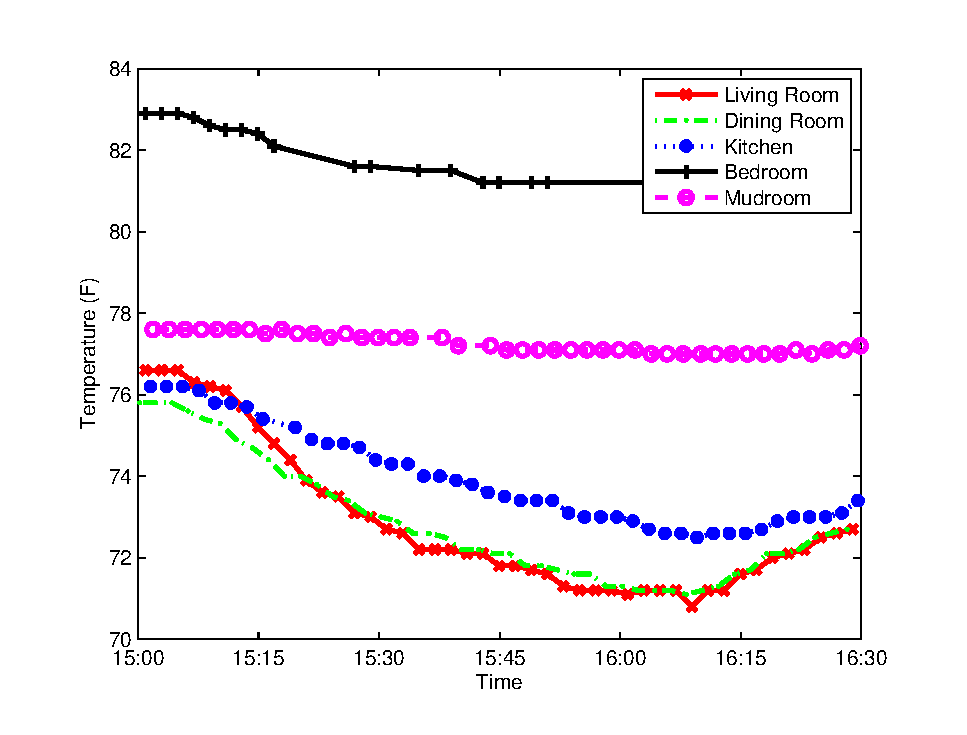
\includegraphics[width=0.6\columnwidth]{fig/houseTempRes.eps}
  \caption[Temperature Response of Conditioned and Unconditioned
    Rooms]{Temperature response of both conditioned and unconditioned rooms as
    the active zone temperature is dropped from 76 to 72.}
  \label{fig:houseTempRes}
\end{figure}

In order to better understand these results, Figure~\ref{fig:airflowBar}
illustrates how effective the active registers were at activating and
de-activating the red and blue zones.  It is clear from this figure that the
greatest airflow in a zone is obtained when the registers in the other zone are
closed.  However, air flow to the inactive zone does not stop, nor does it all
get directed to the active zone.  In future work, we expect an improved active
register system to produce better energy saving and thermal insulation results.

\begin{figure}[ht]
  \centering
  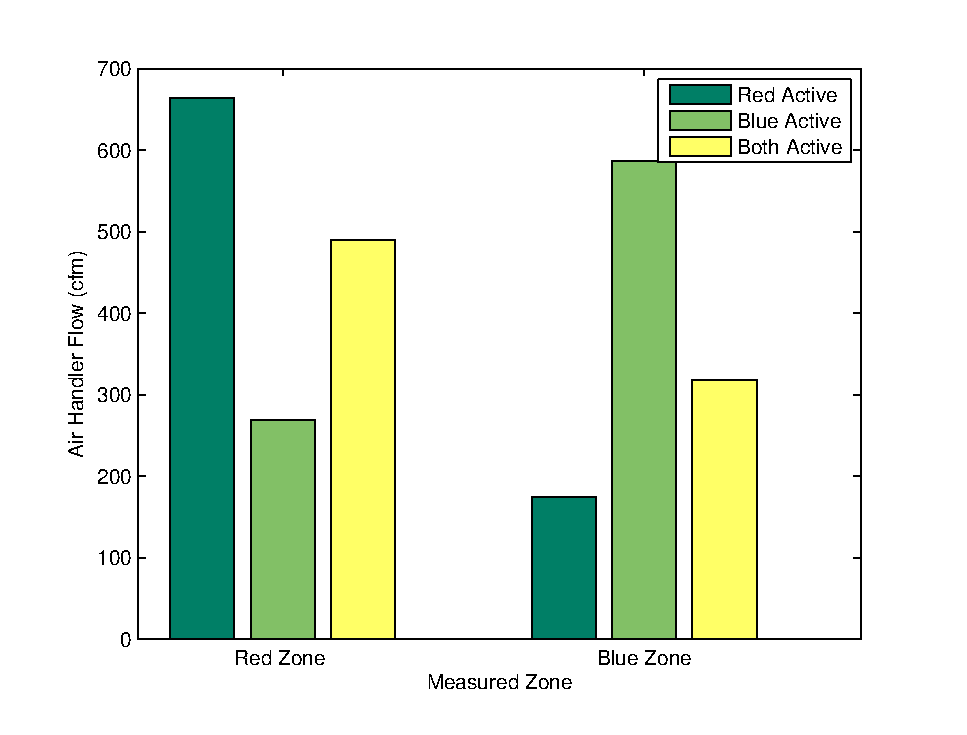
\includegraphics[width=0.6\columnwidth]{fig/airflowBar.eps}
  \caption[Effect of Zoning on Airflow]{Activating different zones does not
    redirect all air flow from one zone to another, but does affect air flow
    substantially.}
  \label{fig:airflowBar}
\end{figure}

\section{Thermal Modeling}
\label{sec:thermalModelingResults}

%% analyze and compare results from all of the models.  Give multiple graphs,
%% including example traces and overall error.  It can also include the
%% percentage accuracy graph that we discussed today.  

We compare the three iterations of our model described in section 5 using 21
days worth of data tested with 10-fold cross validation which involves randomly
dividing the 21 days of data into ten equal sets, training the model using nine
of those sets, and testing with the remaining set. All combinations of nine sets
for training and one set for testing are used. The 21 days we have selected for
model development and testing have been sampled from 3 months worth of data
between October and December 2011. Using the training data, we develop the
$\beta$ values for the model. We then use these values with the $\alpha$ value
scheme dictated by the model iteration in order to predict temperatures when the
system turns on.

\subsection{Prediction}
Our predictions assume that temperature grows linearly when the system turns on
as a result of the current damper configuration and the previous weather
patterns estimated through $\alpha$. Though temperature dynamics within a
building are often nonlinear, we find a reasonable estimate by predicting
temperature linearly into the future. This is because the temperature and
airflow of the system operate within a narrow regime, making it reasonable to
approximate change with a linear model. An example of a prediction 30 minutes
into the future is shown in Figure~\ref{fig:expred}. Here, the blue lines
represent the actual temperatures and the red line plots our prediction. The
solid blue line shows the temperature when the system is off, and the red/blue
dashed lines show the predicted/actual temperatures when the system has just
turned on.

\begin{figure}
\begin{center}
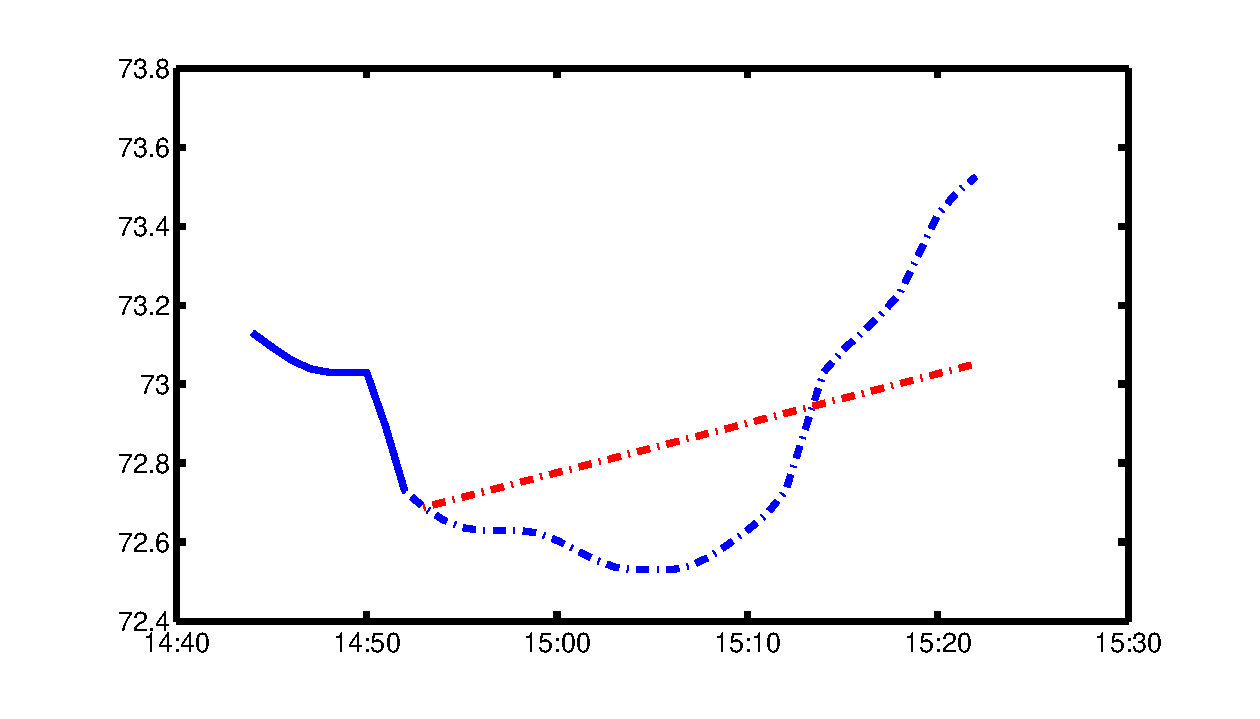
\includegraphics[width=0.6\columnwidth]{fig/ExamplePrediction.eps}
\end{center}
\caption[An example of a temperature prediction.]{An example of a prediction
  made for temperature up to 30 minutes after the system turns on. The solid
  blue line shows the actual temperature when the system is off; the dashed blue
  line shows the actual temperature when the system is on; and the dashed red
  line shows temperature predicted after the system has just turned on.}
\label{fig:expred}
\end{figure}

\subsection{Error Metric}
\label{sec:errormetric}
One difficulty in determining the effectiveness of these models is that we aim
to use them to predict temperatures at more than one timestep into the
future. This involves calculating predictions at each point that the system is
on, up to $t$ minutes into the future until the system turns off again.

The error metric that we have chosen for this comparison is to determine the
distribution of prediction error as we predict $t$ minutes into the future. For
each minute, $t$, we calculate the mean and standard deviation of the prediction
errors $t$ minutes away from the initial time. The results from these analyses
for the static $\alpha$, dynamic $\alpha$, and adjacency model are shown in
Figure~\ref{fig:staticerror}, Figure~\ref{fig:dynamicerror}, and
Figure~\ref{fig:adjerror} respectively. These results are calculated on a
per-sensor basis for each of the 12 sensors in the 7 rooms of the building.

Visually examining the error distributions highlights a few important things
about the model. One is that the variance of the errors tends to increase as we
predict further into the future. The error can get quite large in some places,
particularly in the dynamic $\alpha$ model. However, most of the values for each
model remain within 2 degrees for the 30 minute prediction. This is a reasonable
interval with which to enable the control of the system that we aim to
accomplish.

The results from this analysis also indicate that the simple, pooled $\alpha$
model performs better than the dynamic model. This may be counterintuitive since
weather tends to change significantly throughout the day. However, because of
the window we are looking at and the narrow range of temperature change, it is
reasonable that this model should perform well. It also has the added benefit of
being computable and easy to implement within a control setting.

\begin{figure}
\centering
\begin{tabular}{cc}
\begin{minipage}{\linewidth}
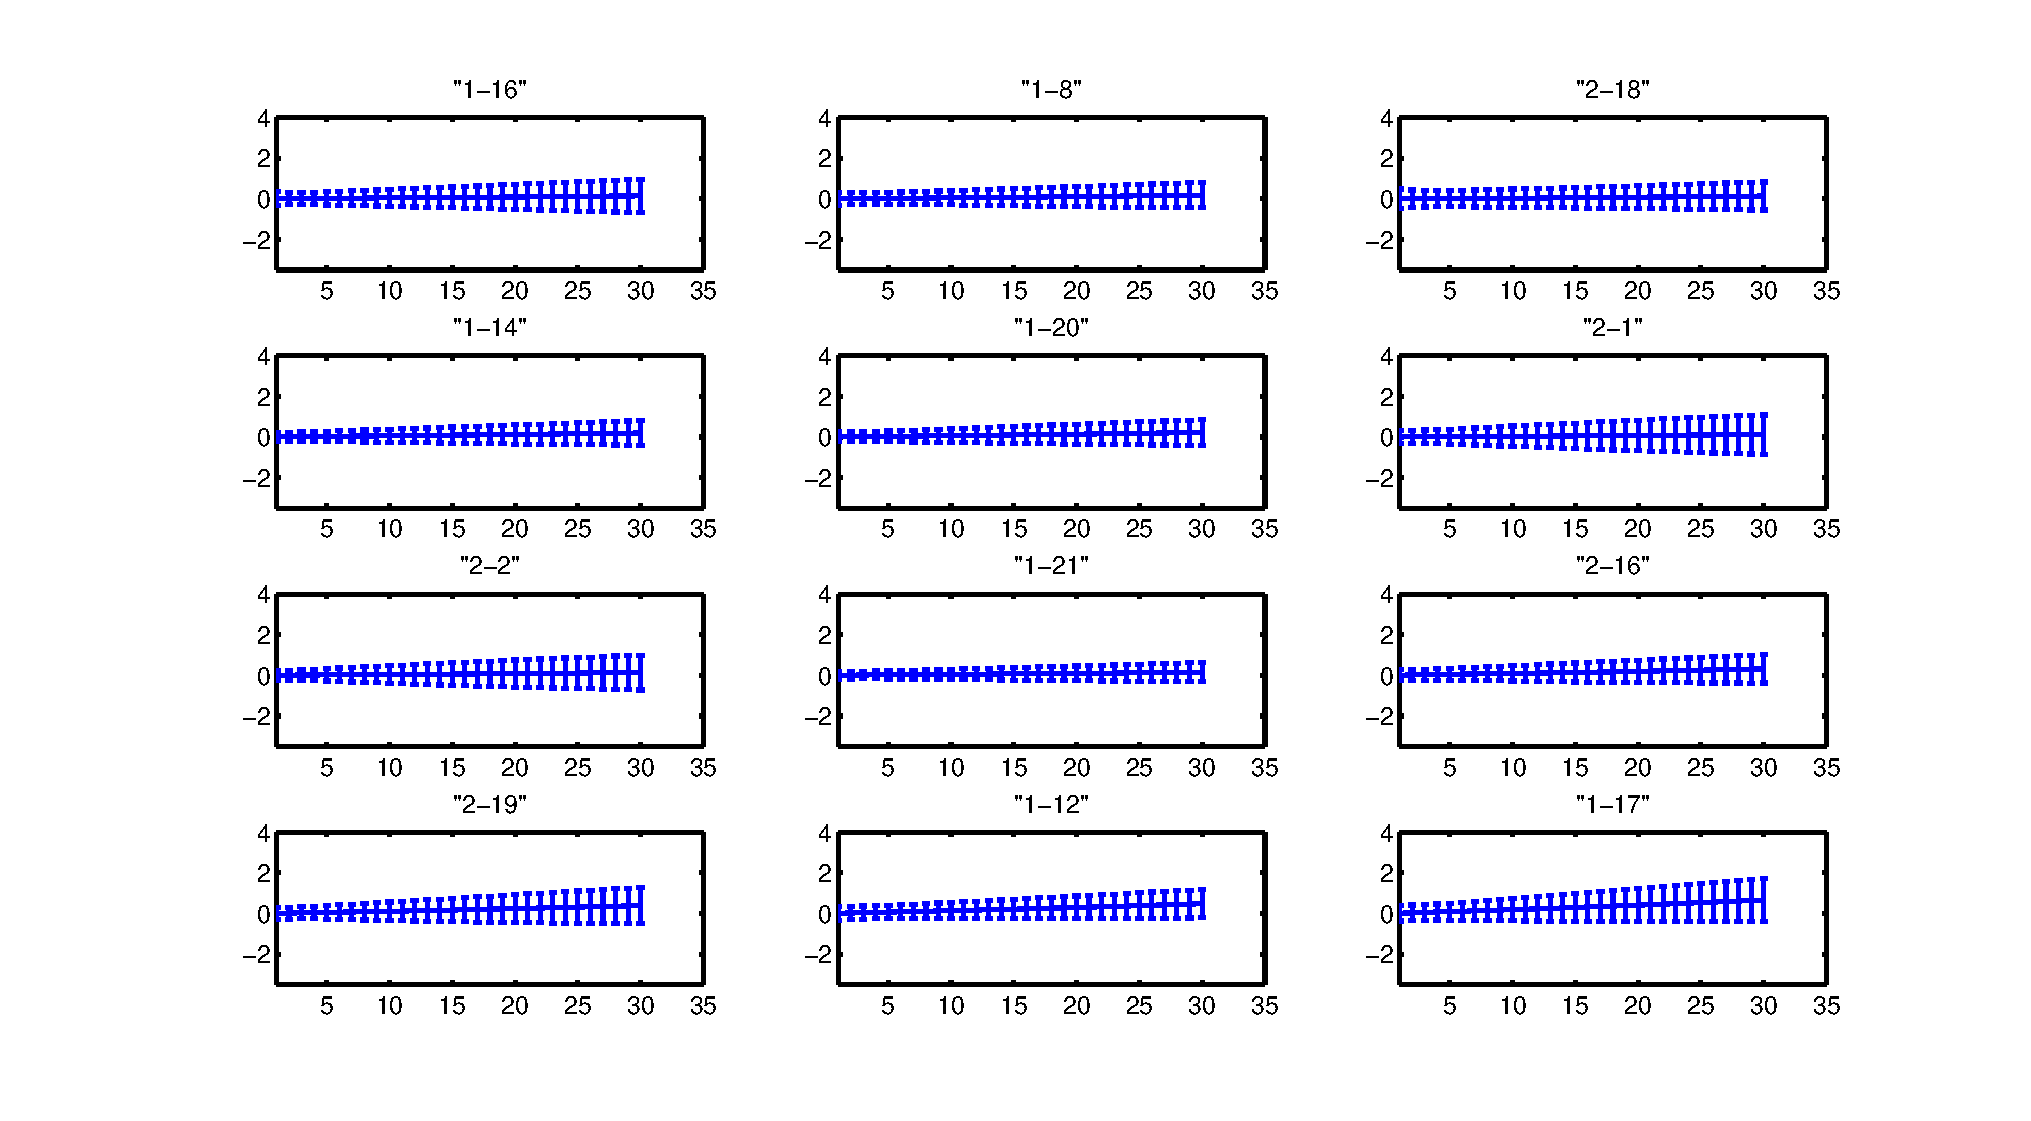
\includegraphics[width=0.6\columnwidth]{fig/PooledSingleError.eps}
\caption[Error distribution for the static $\alpha$ model.]{Error distribtuions
  for the static $\alpha$ model, up to 30 minutes into the future. The locations
  of the twelve sensors are presented in Figure~\ref{fig:floorplan}}
\label{fig:staticerror}
\end{minipage}\\
\begin{minipage}{\linewidth}
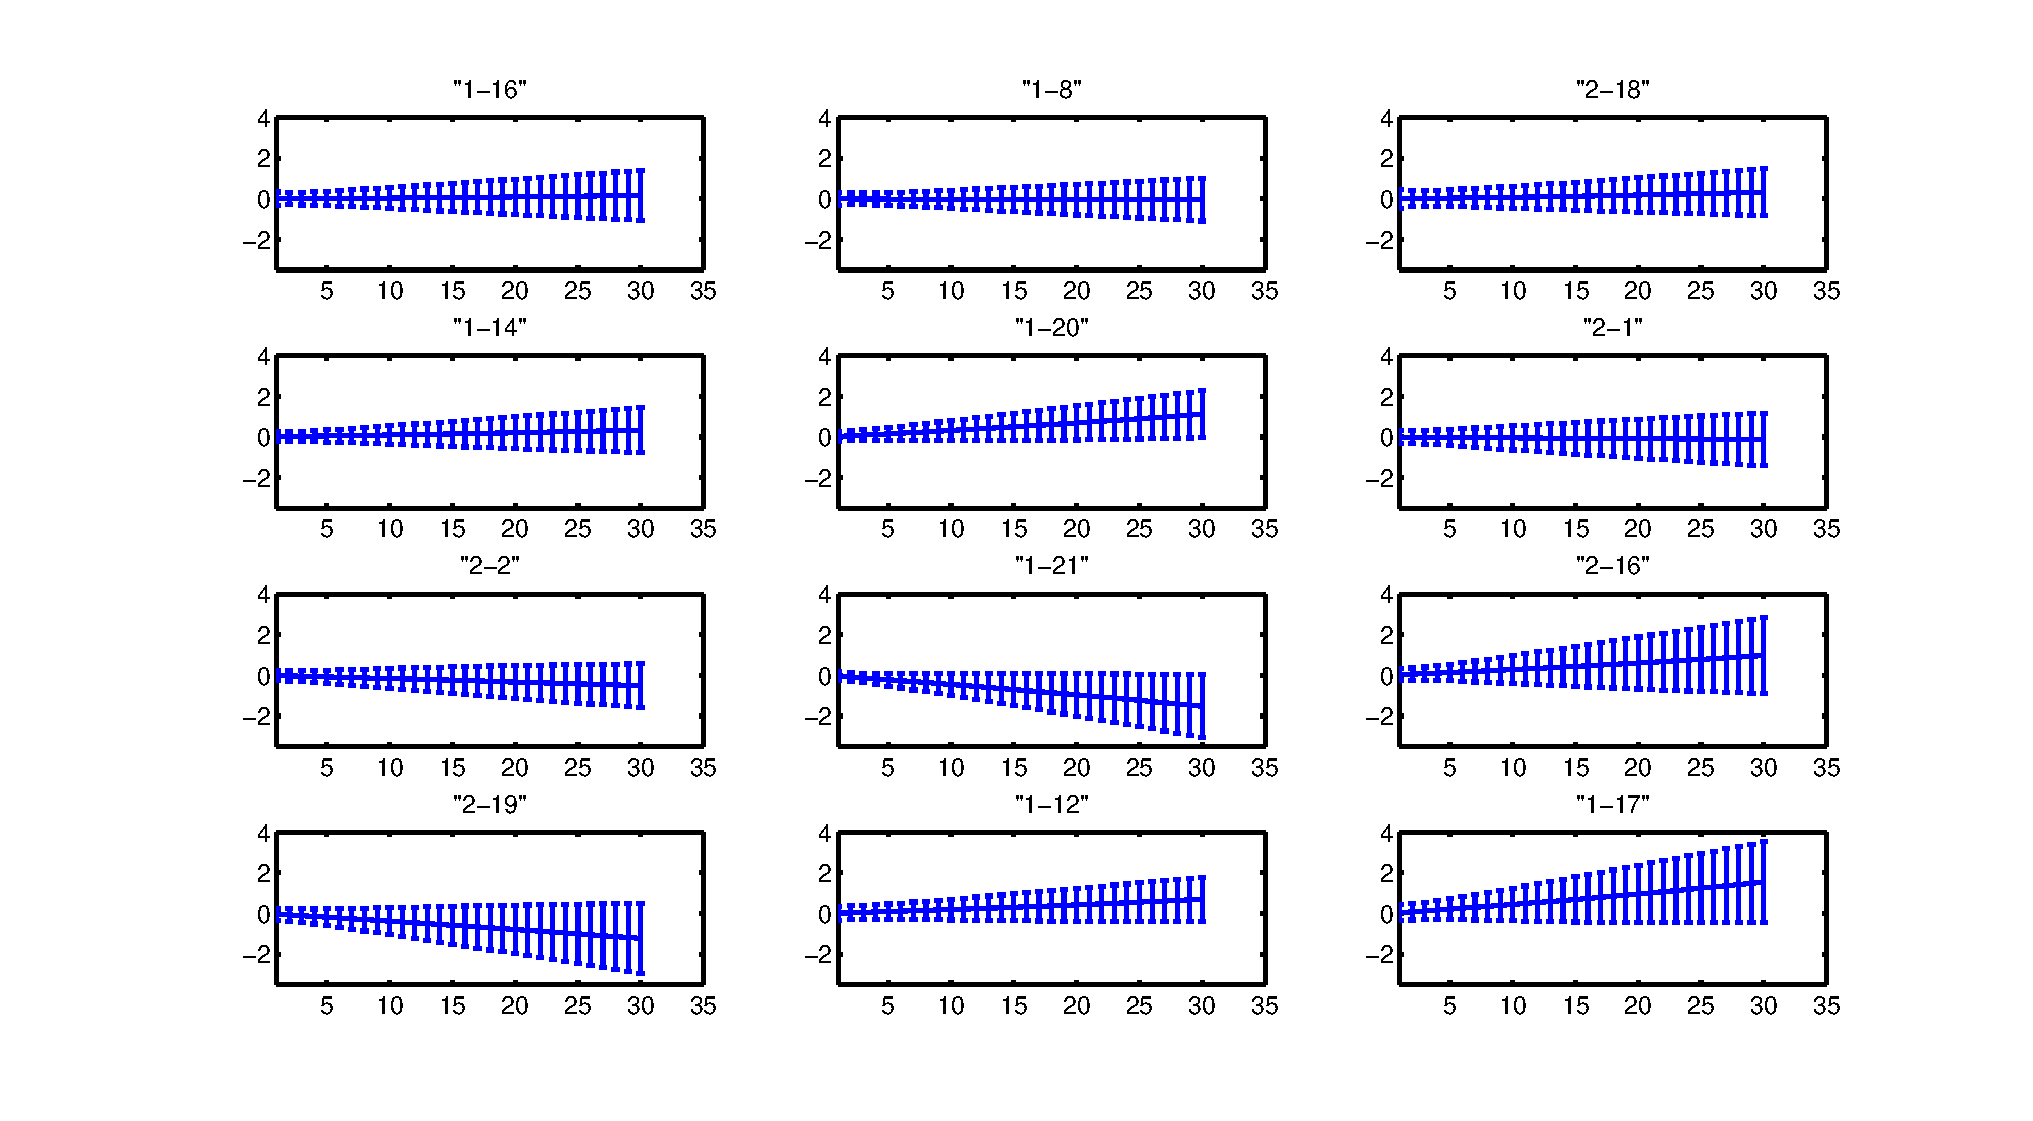
\includegraphics[width=0.6\columnwidth]{fig/DynSingleError.eps} 
\caption[Error distribution for the dynamic $\alpha$ model.]{Error distributions
  for the dynamic $\alpha$ model, up to 30 minutes into the future. The
  locations of the twelve sensors are presented in Figure~\ref{fig:floorplan}}
\label{fig:dynamicerror}
\end{minipage}\\
\begin{minipage}{\linewidth}
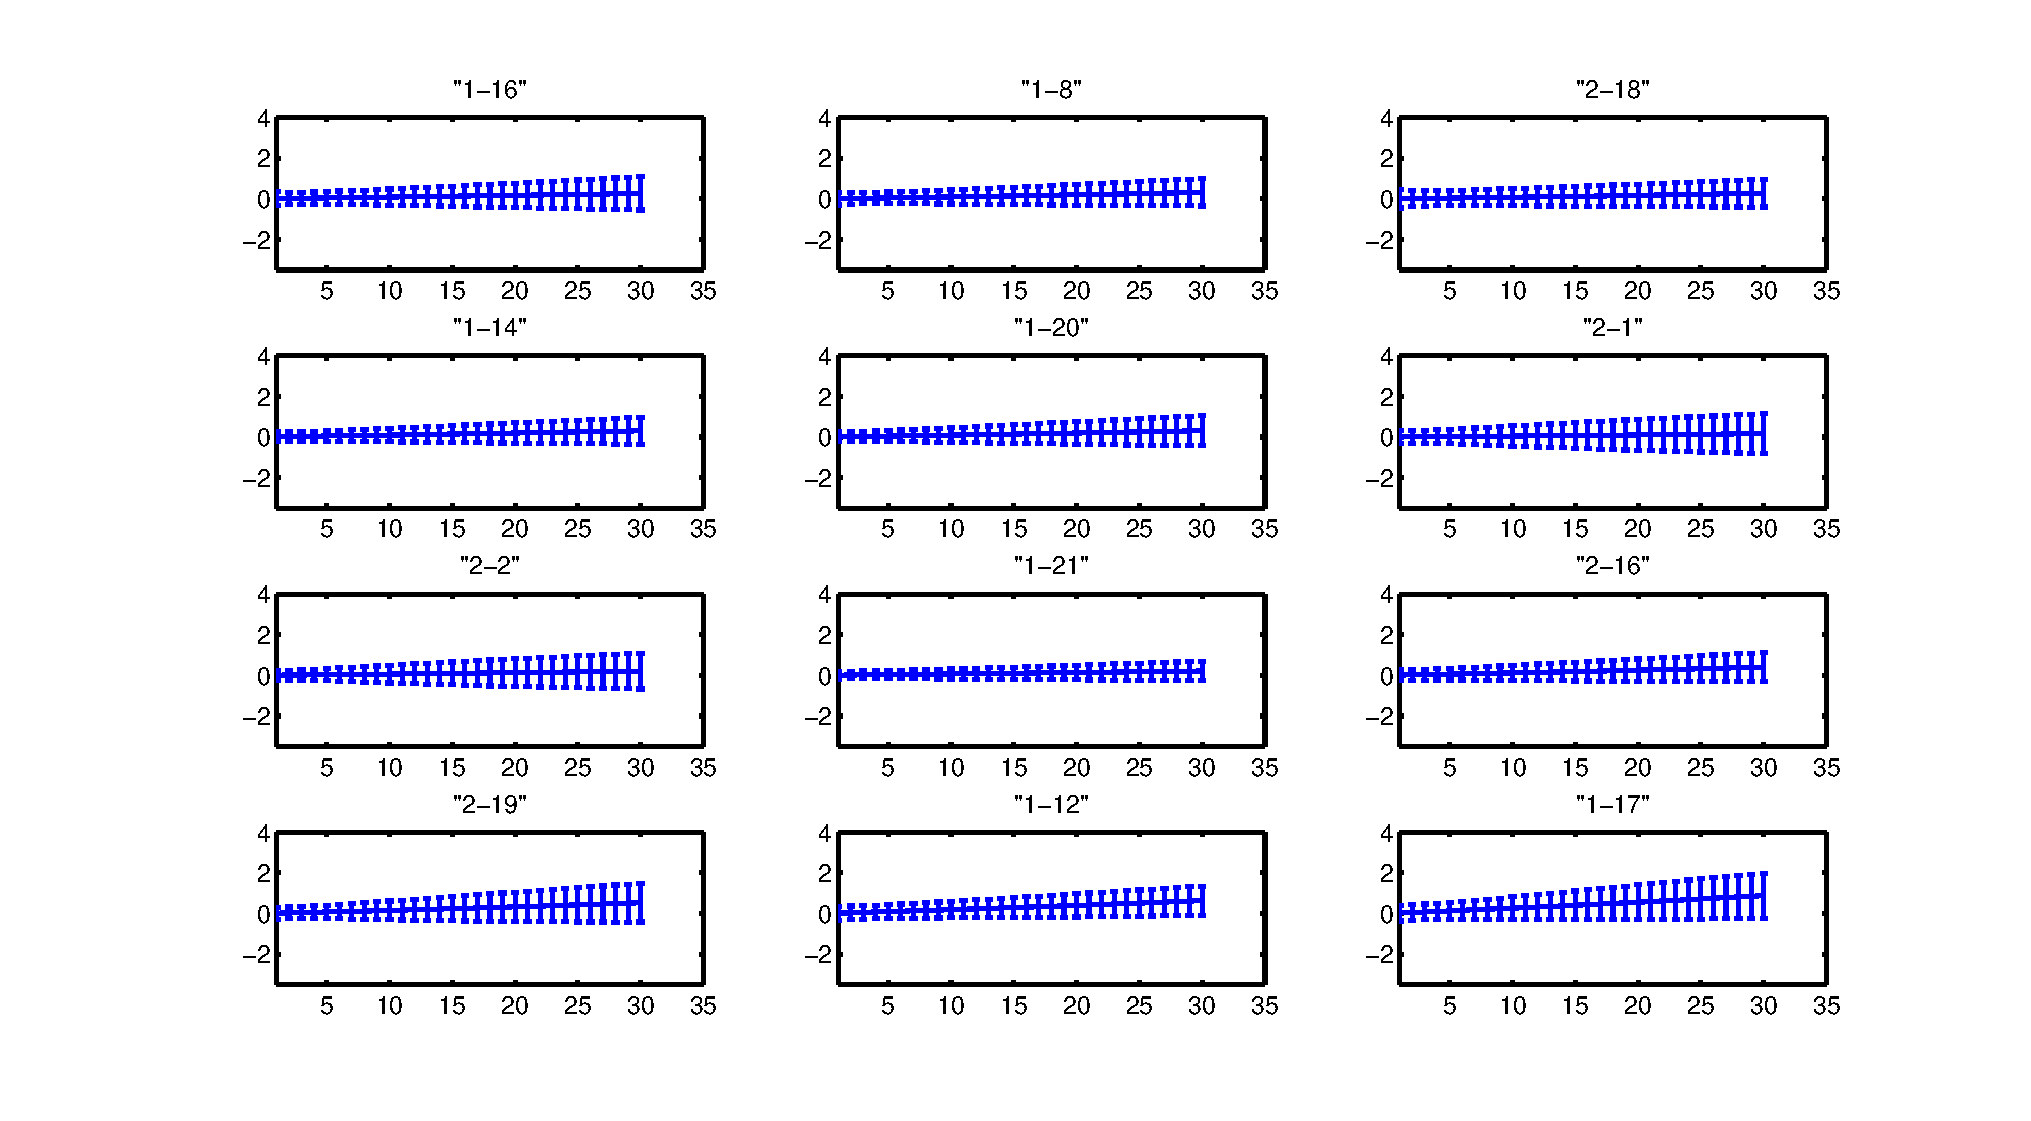
\includegraphics[width=0.6\columnwidth]{fig/PooledAdjError.eps}
\caption[Error distribution for the adjacency model.]{Error distributions for
  the adjacency model, up to 30 minutes into the future. The locations of the
  twelve sensors are presented in Figure~\ref{fig:floorplan}}
\label{fig:adjerror}
\end{minipage}
\end{tabular}
\end{figure}
